\begin{center}
\Huge
Optimering
\end{center}

\section*{Optimering}
\stepcounter{section}

Vi vil introducere dette emne med en række eksempler. 
\begin{exa}
Vi har $50m$ hegn og vi skal lave en indhegning til en hønsegård. Vi vil gerne have glade høns, så vi ønsker selvfølgelig, at arealet af indhegningen er maksimeret. En af indhegningens sider er op ad et hus, og vi vil gerne have en rektangulær indhegning. Derfor skal vi kun have tre sider i vores indhegning. Indhegningen kan ses på Fig. \ref{fig:indh}
\begin{figure}[H]
\centering
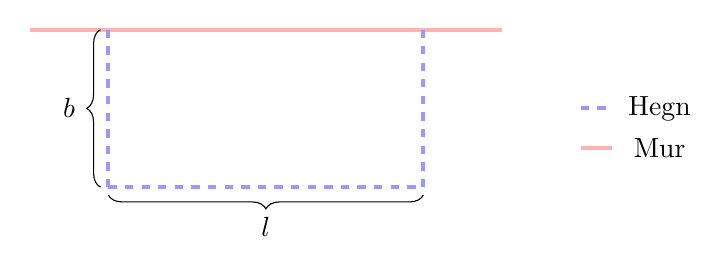
\begin{tikzpicture}
\draw[line width = 0.5mm,color=red!30] (-3,0) -- (3,0);
\draw[line width = 0.5mm, dashed, color = blue!40] (-2,0) -- (-2,-2);
\draw[line width = 0.5mm, dashed, color = blue!40] (-2,-2) -- (2,-2);
\draw[line width = 0.5mm, dashed, color = blue!40] (2,-2) -- (2,0);
\draw[line width = 0.5mm, dashed, color = blue!40] (4,-1) -- (4.4,-1);
\draw[line width = 0.5mm, color=red!30] (4,-1.5) -- (4.4,-1.5);
\node at (5,-1) {Hegn};
\node at (5,-1.5) {Mur};
\draw [decorate,decoration = {brace,mirror,amplitude = 5pt}] (-2.1,-0.0) --  (-2.1,-2);
\draw [decorate,decoration = {brace,mirror,amplitude = 5pt}] (-2,-2.1) --  (2,-2.1);
\node at (-2.5,-1) {$b$};
\node at (0,-2.5) {$l$};
\end{tikzpicture}
\caption{Hønsegård}
\label{fig:indh}
\end{figure}
Vi ved, at arealet af hønsegården er givet ved 
\begin{align}\label{eq:areal}
A(l,b) = lb,
\end{align}
samt at den samlede hegnslængde er givet ved 
\begin{align}\label{eq:hegnsl}
L(l,b) = 2b+l = 50m,
\end{align}
som er fastlagt til $50m$, da det er længden af det hegn, vi har til rådighed. Vi kan isolere længden $l$ i udtrykket \eqref{eq:hegnsl} som
\begin{align}\label{eq:lsomfb}
l = 50-2b.
\end{align}
Dette kan vi nu sætte ind i \eqref{eq:areal} for at få et udtryk for arealet $A(l,b)$, der kun afhænger af $b$:
\begin{align*}
A(l,b) = lb = (50-2b)b = 50b-2b^2.
\end{align*}
Grafen for $A(b)$ er tegnet i Fig. \ref{fig:honsegraf}
\begin{figure}[H]
	\centering
	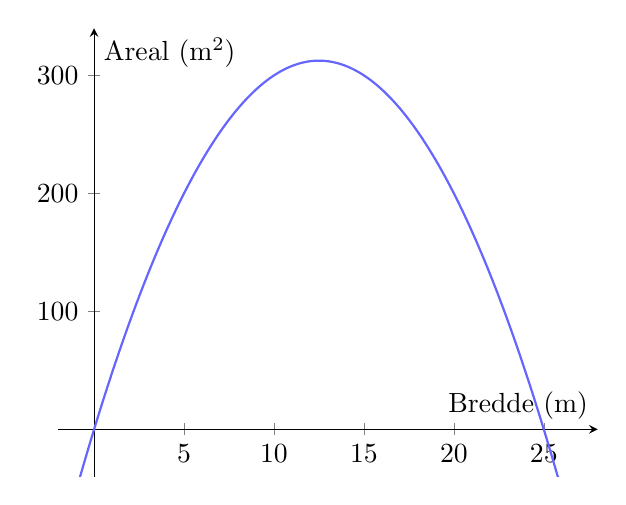
\begin{tikzpicture}
		\begin{axis}[
		axis lines = middle, 
		xmin = -2, xmax = 28, 
		ymin = -40, ymax = 340,
		xlabel = {Bredde (m)},
		ylabel = {Areal (m$^2$)}		
		]
			\addplot[color = blue!60, thick, samples = 1000, domain = -2:28] {50*x-2*x^2};
		\end{axis}
	\end{tikzpicture}
	\caption{Areal $A$ af hønsegård som funktion af bredde $b$.}
	\label{fig:honsegraf}
\end{figure}

Af Fig. \ref{fig:honsegraf} ser det ud som om arealet er maksimeret omkring $b=12m$, men vi vil gerne finde den eksakte maksimerende bredde. Derfor vil vi finde toppunktet for andengradspolynomiet $A(b) = 50b-2b^2$. Vi finder derfor den afledede funktion
\begin{align*}
A'(b) = 50-4b,
\end{align*}
og vi sætter denne lig nul for at finde ud af, hvor tangenthældningen er $0$. Vi får altså
\begin{align*}
A'(b) = 50-4b = 0 &\Leftrightarrow 50=4b\\
&\Leftrightarrow 12,5=b,
\end{align*}
hvilket også stemmer nogenlunde overens med aflæsningen fra Fig. \ref{fig:honsegraf}. Udtrykket \eqref{eq:lsomfb} giver os et udtryk for længden $l$ udtrykt ved bredden $b$. Altså må den maksimerende længde være 
\begin{align*}
l = 50-2\cdot 12,5 = 25m,
\end{align*}
altså skal længden af buret være $25m$ i det maksimerende tilfælde. Til slut bestemmer vi det maksimerende areal ved brug af \eqref{eq:areal} som
\begin{align*}
A((12,5),25) = 12,5\cdot25 = 312,5m^2,
\end{align*}
som altså er det maksimalt opnåelige areal til hønseindhegningen. 
\end{exa}
\begin{exa}
Vi forestiller os, at vi har en kasse med kvadratisk bund med areal $b^2$ og højde $h$. Vi ønsker at minimere materialeforbruget til kassen, når kassen ikke skal have et låg, og rumfanget af kassen skal være $4m^3$. Kassen kan ses på Fig. \ref{fig:kasse}
\begin{figure}[H]
\centering
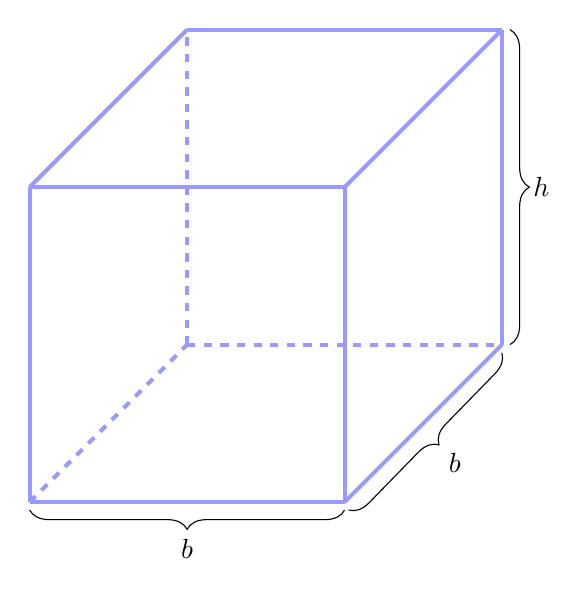
\begin{tikzpicture}
\draw[line width = 0.5mm,  color = blue!40] (0,0) -- (0,4);
\draw[line width = 0.5mm,  color = blue!40] (0,0) -- (4,0);
\draw[line width = 0.5mm,  color = blue!40] (4,0) -- (4,4);
\draw[line width = 0.5mm,  color = blue!40] (0,4) -- (4,4);

\draw[line width = 0.5mm,  color = blue!40] (0,4) -- (2,6);
\draw[line width = 0.5mm,  color = blue!40] (4,4) -- (6,6);
\draw[line width = 0.5mm,  color = blue!40] (6,6) -- (6,2);

\draw[line width = 0.5mm,  color = blue!40] (4,0) -- (6,2);
\draw[line width = 0.5mm,  color = blue!40] (2,6) -- (6,6);

\draw[line width = 0.5mm, dashed,  color = blue!40] (0,0) -- (2,2);
\draw[line width = 0.5mm, dashed,  color = blue!40] (2,2) -- (2,6);
\draw[line width = 0.5mm, dashed,  color = blue!40] (2,2) -- (6,2);

\draw [decorate,decoration = {brace,mirror,amplitude = 7pt}] (0,-0.1) --  (4,-0.1);
\draw [decorate,decoration = {brace,mirror,amplitude = 7pt}] (4.05,-0.1) --  (6,1.9);
\draw [decorate,decoration = {brace,mirror,amplitude = 7pt}] (6.1,2) --  (6.1,6);

\node at (2,-0.6) {$b$};
\node at (5.4,0.5) {$b$};
\node at (6.5,4) {$h$};
\end{tikzpicture}
\caption{Kasse uden låg med højde $h$ og grundfladeareal $b^2$.}
\label{fig:kasse}
\end{figure}
Fremgangsmåden er tilsvarende den, vi opstillede til eksemplet med hønsegården. Vi opstiller altså de variabelsammenhænge, vi har. Det samlede overfladeareal er givet ved
\begin{align*}
O(b,h) = b^2+4bh,
\end{align*}
hvilket er størrelsen, vi skal minimere. Kassens rumfang er givet ved
\begin{align*}
R(b,h) = b^2h = 4.
\end{align*}
Vi kan isolere $h$ i dette udtryk og få
\begin{align*}
h = \frac{4}{b^2}.
\end{align*}
Dette sættes ind i udtrykket for det samlede overfladeareal:
\begin{align*}
O(b,h) = b^2+ 4bh = b^2 + \frac{4\cdot4b}{b^2} = b^2+\frac{16}{b}.
\end{align*}
Dette skal vi maksimere. Grafen for $O(b)$ kan ses på Fig. \ref{fig:kassegraf}.
\begin{figure}[H]
	\centering
	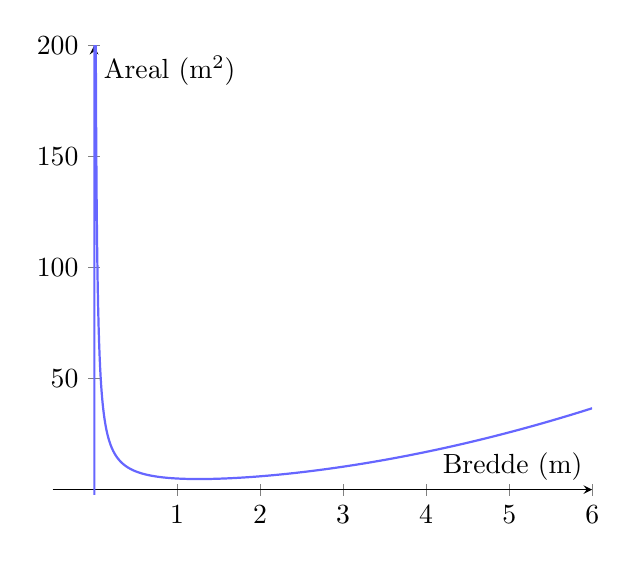
\begin{tikzpicture}
		\begin{axis}[
		axis lines = middle, 
		xmin = -0.5, xmax = 6, 
		ymin = -2, ymax = 200,
		xlabel = {Bredde (m)},
		ylabel = {Areal (m$^2$)}		
		]
			\addplot[color = blue!60, thick, samples = 1000, domain = -0.2:6] {x^2+4/x};
		\end{axis}
	\end{tikzpicture}
	\caption{Overfladeareal $O$ som funktion af bredde $b$.}
	\label{fig:kassegraf}
\end{figure}

Af grafen kan det ses, at der er et lokalt minimum omkring en bredde $b=2m$, men det er ikke et globalt minimum. Dog kan vi selvfølgelig ikke have negative bredder, så vi er kun interesseret i den positive halvakse. Vi ønsker som før at finde punktet, hvor tangenthældningen er $0$, så vi differentierer overfladearealet og sætter lig $0$:
\begin{align*}
O'(b) = 2b-\frac{16}{b^2}=0&\Leftrightarrow 2b^3-16=0\\
						&\Leftrightarrow 2b^3 = 16\\
						&\Leftrightarrow b^3 = 8\\
						&\Leftrightarrow b = \sqrt[3]{8} = 2,
\end{align*}
og den bredde $b$, der minimerer overfladearealet er $b=2m$. Da $h=4/b^2$, så er den minimerende højde $h=4/2^2=1m$ og det minimerede overfladeareal er givet ved
\begin{align*}
O(2,1) = 2^2+4\cdot 2\cdot 1 = 12m^2
\end{align*}
\end{exa}

\section*{Opgave 1}
\begin{enumerate}[label=\roman*)]
\item Løs problemet med hønseburet fra Eksempel 2.1, men nu hvor den samlede længde på hegnet er $20m$
\item Løs problemet med kassen fra Eksempel 2.2, men nu hvor kassen skal have et låg.
\item En landmand skal lave en indhegning på en mark. Den skal være kvadratisk, og han har $5000m$ hegn. Hvad skal dimensionerne på hegnet være for at maksimere arealet af indhegningen? Hvad er det størst mulige areal?
\end{enumerate}